% !TeX spellcheck = cs_CZ
{\tikzset{external/prefix={tikz/FYZI/}}
 \tikzset{external/figure name/.add={ch13_}{}}
%---------------------------------------------------------------------------------------------------
% file fey1ch16.tex
%---------------------------------------------------------------------------------------------------
%=========================== Kapitola: Relativistická energie a hybnost ===========================
\chapter{Relativistická energie a hybnost}\label{fyz:IchapXVI}
\minitoc
  \section{Relativita a filozofové}\label{fyz:IchapXVIsecI}
    V této kapitole budeme pokračovat v diskuzi o Einsteinově a Poincaréově principu relativity, 
    jeho vlivech na názory fyziků a na jiná odvětví lidského myšlení.
    
    Poincaré formuloval své poznatky následujícím způsobem: „Podle principu relativity musí být 
    zákony fyzikálních jevů stejné pro pozorovatele, který se nepohybuje, i pro toho, který je 
    vzhledem k němu v rovnoměrném pohybu, takže nemáme, a pravděpodobně ani nemůžeme mít, žádné 
    prostředky k rozpoznání toho, zda se nacházíme v takovémto pohybu nebo ne.“
    
    Když se objevila tato myšlenka, způsobila mezi filozofy velký rozruch, zejména mezi „filozofy z 
    koktejlových večírků“. Konstatovali: „Ó, to je velmi jednoduché, Einsteinova teorie říká, že 
    všechno je relativní!“ Skutečně, až překvapivě mnoho filozofů, a nejen těch z koktejlových 
    večírků (ale abychom je neurazili, budeme hovořit pouze o „filozofech z koktejlových večírků“), 
    říká: „To, že vše je relativní, vyplývá z Einsteinovy teorie a má to mimořádný vliv na naše 
    myšlení.“ Jako dodatek říkají: „Ve fyzice bylo dokázáno, že jevy závisejí na naší vztažné 
    soustavě.“ Často to slýcháme, ale těžko lze zjistit, co se tím myslí. Pravděpodobně se pod 
    vztažnými soustavami, na něž se tak originálně odvolávají, myslí souřadnicové soustavy, jež 
    používáme v teorii relativity. Proto skutečnost, že „věci závisejí na naší vztažné soustavě“, 
    by měl mít údajně ten velký vliv na současné myšlení. Je možné se podivit proč, neboť 
    koneckonců, že se věci různě jeví v závislosti na hledisku, které zaujmeme, je myšlenka tak 
    jednoduchá, že k jejímu objevení určitě nebylo třeba podstoupit všechny těžkosti, abychom 
    objevili fyzikální teorii relativity. Každý jistě ví, že to, co vidí, závisí na jeho vztažné 
    soustavě, neboť přicházejícího chodce vidí nejprve zepředu, potom zezadu. Velká část filozofie, 
    která údajně pochází z teorie relativity, neobsahuje nic hlubšího, než to, že „osoba vypadá 
    jinak zepředu a jinak zezadu“. Známý příběh o tom, jak více slepců popsalo slona, přitom každý 
    jinak, je snad dalším příkladem teorie relativity z hlediska filozofie.
    
    Ale v teorii relativity určitě musí být něco hlubšího než jednoduchá poznámka, že „člověk 
    vypadá jinak zepředu a jinak zezadu“. Relativita je něco víc, neboť \emph{pomocí ní můžeme 
    učinit jisté předpovědi}. Bylo by velmi pozoruhodné, kdybychom pouze na základě tak 
    jednoduchého poznatku mohli předpovídat přírodní jevy.
    
    Existuje jiná škola filozofů, jímž se zdá být teorie relativity, podle níž nemůžeme určit naši 
    absolutní rychlost, aniž bychom se dívali ven, nepohodlná. Říkají: \uv{Je samozřejmé, že 
    nemůžeme měřit naši rychlost, aniž bychom se podívali ven. Je jasné, že hovořit o rychlosti, 
    aniž bychom se podívali ven, \emph{nemá smysl}}; fyzici jsou dost hloupí, když si mysleli opak, 
    ale nyní se jim ujasnilo, že je to tak. „Kdybychom si my, filozofové, byli uvědomili, jaké 
    problémy mají fyzici, mohli jsme už dávno pomocí rozumové úvahy rozhodnout, že je nemožné říci, 
    jak rychle se někdo pohybuje, aniž by se díval kolem sebe. Mohli jsme vykonat obrovský kus 
    práce ve fyzice.“ Takovéto filozofy, bojující na periférii a pokoušející se nám něco říci, máme 
    vždy kolem sebe, ale ti nikdy nepochopili složitost a hloubku problému.
    
    Naše neschopnost určit absolutní pohyb vyplývá z \emph{experimentu} a není výsledkem pouhého 
    myšlení, což můžeme snadno ilustrovat. Za prvé, Newton věřil, že nelze určit rychlost pohybu, 
    pohybujeme-li se rovnoměrně po přímce. Skutečně, Newton jako první zformuloval princip 
    relativity. Proč nenadělali filozofové takový rozruch, že „vše je relativní“ (nebo nějak 
    podobně) ještě v době Newtona? Protože až do doby vzniku Maxwellovy teorie nebyly známy takové 
    fyzikální zákony, na jejichž základě by se zdálo, že \emph{lze} určit rychlost pohybu bez 
    pohledu ven. \emph{Experimentálně} se brzy zjistilo, že to \emph{není možné}.
    
    Je z filozofického hlediska absolutně a definitivně nevyhnutelné, aby nebylo možné zjistit 
    rychlost pohybu bez pohledu ven? Jedním z důsledku relativity byl vznik filozofie, podle které: 
    „Definovat lze jen to, co lze měřit!“ Protože je zřejmé, že rychlost nelze měřit, aniž bychom 
    neviděli vzhledem k čemu ji měříme, proto je jasné, že absolutní rychlost \emph{nemá smysl}. 
    Fyzici by si měli uvědomit, že mohou hovořit pouze o tom, co mohou měřit.“ Ale \emph{to je celý 
    problém}: Zda \emph{lze definovat} absolutní rychlost, nebo ne, je tatáž otázka, jako zda lze 
    nebo nelze \emph{experimentálně zjistit} pohyb bez pohledu ven. Jinak řečeno, zda něco lze nebo 
    nelze měřit, není možné rozhodnout a priori pouhým myšlením; rozhodnout lze jen pomocí 
    experimentu. Našli bychom málo filozofů, kteří by při vědomí, že rychlost světla je \SI{300 
    000}{\km\per\s}, klidně prohlásili, že jestliže světlo letí vzhledem k autu rychlostí \SI{300 
    000}{\km\per\s}  a auto má rychlost \SI{200 000}{\km\per\s}, že toto světlo proletí kolem 
    stojícího pozorovatele také rychlostí \SI{300 000}{\km\per\s}. To je pro ně šokujícím faktem. 
    Právě ti, pro něž je relativita tak samozřejmá, zjistí, když přijde na konkrétní fakt, že to 
    není tak docela jasné.
    
    Nakonec, existuje dokonce filozofie, která tvrdí, že bez pohledu ven nelze určit žádný pohyb. 
    Ve fyzice to prostě neplatí. Pravda, \emph{rovnoměrný přímočarý} pohyb nemůžeme zaregistrovat. 
    Kdyby se celý pokoj \emph{otáčel} určitě bychom to věděli, neboť by to každého hodilo na stěnu 
    - uplatnily by se všechny odstředivé efekty. Otáčení Země kolem osy lze určit bez pohledu na 
    hvězdy, například pomocí tzv. \textbf{Foucaultova kyvadla}. Proto není pravda, že „vše je 
    relativní“ - je to jen pohyb \emph{rovnoměrnou rychlostí}, který nelze zjistit bez pohledu ven. 
    Rovnoměrné \emph{otáčení} kolem pevné osy zjistit lze. Jestliže to řekneme nějakému filozofovi, 
    je velmi zklamán, že věc skutečně nechápe, neboť jemu se zdá být nemožné určit rotaci kolem osy 
    bez pohledu ven. Je-li někdo docela dobrý filozof, po nějaké době se může vrátit a říci: 
    „Rozumím - něco jako absolutní otáčivý pohyb skutečně nemáme; ve skutečnosti se otáčíme 
    \emph{vzhledem ke hvězdám}. Takže odstředivá síla musí být způsobena vlivem hvězd na objekty.“
    
    Podle toho, co víme, je to pravda. Dnes neumíme říci, jestli by byla odstředivá síla, kdyby 
    nebyly kolem hvězdy a mlhoviny. Nejsme schopni provést experiment, při němž bychom odstranili 
    všechny mlhoviny a pak změřili naši rotaci, proto o tom prostě neumíme nic říci. Musíme 
    připustit, že filozof může mít pravdu. Přijde proto nadšený zpět a řekne: „Je to naprosto 
    nutné, aby svět byl uspořádán tímto způsobem. \emph{Absolutní} otáčení nemá smysl, otáčení je 
    pouze relativní \emph{vzhledem} k mlhovinám.“ My mu pak odpovíme: „Příteli, je tedy nebo není 
    zřejmé, že rovnoměrná rychlost po přímce, relativní \emph{vzhledem k mlhovinám} se neprojeví 
    žádným účinkem uvnitř auta?“ Nyní, kdy pohyb není absolutní, aleje pohybem \emph{relativním k 
    mlhovinám} je toto základní otázka a zároveň taková, na niž lze odpovědět jen pomocí 
    experimentu.
    
    Jaké jsou tedy filozofické vlivy teorie relativity? Omezíme-li se na vlivy v tom smyslu, 
    \emph{jaké nové myšlenky a podněty} vyplývají pro fyziku z principu relativity, mohli bychom je 
    popsat následujícím způsobem: První objev je v podstatě to, že dokonce i ty ideje, které byly 
    velmi dlouho uznávány, a které byly velmi přesně ověřeny, mohou být mylné. To, že jsou 
    Newtonovy zákony chybné, byl po mnoha letech, kdy se zdály být přesné, samozřejmě šokující 
    objev. Je jasné, že příčinou nejsou špatné experimenty. Byly však provedeny pouze v omezeném 
    rozsahu rychlosti, v tak malém, že relativistické efekty se neprojevily. Nicméně, dnes 
    zaujímáme mnohem pokornější stanovisko k našim fyzikálním zákonům - všechno \emph{může} být 
    špatně!
    
    Za druhé, máme-li systém „podivných“ idejí jako třeba, že čas běží pomaleji pro toho, kdo se 
    pohybuje, není podstatné, zda se nám \emph{líbí}, nebo ne. Jediné, co je třeba respektovat, je 
    zda se tyto ideje shodují s výsledkem experimentu. Stačí, jsou-li „podivné ideje“ potvrzeny 
    \emph{experimentem} a jediným důvodem proč jsme museli rozebírat chod hodin apod., bylo 
    dokázat, že ačkoli je představa dilatace času divná, je v \emph{souladu} s tím, jak měříme čas.
    
    Konečně, je tu třetí podnět, který je trochu techničtější, ale jak se ukázalo, je mimořádně 
    užitečný při studiu ostatních fyzikálních zákonů. Přikazuje \emph{dívat se na symetrii těchto 
    zákonů}, nebo přesněji, hledat způsoby, jak lze tyto zákony transformovat tak, aby zůstaly 
    nezměněny. V teorii vektorů jsme si všimli, že základní pohybové zákony se nemění, otočíme-li 
    souřadnicovou soustavu. Nyní jsme zjistili, že se nemění, když určitým způsobem pomocí 
    Lorentzovy transformace změníme prostorové a časové proměnné. Takže myšlenka studovat strukturu 
    operací, při \emph{níž} se fyzikální zákony nemění, se ukázala být velmi prospěšnou.
    
  \section{Paradox dvojčat}\label{fyz:IchapXVIsecII}
    V pokračování naší diskuze o Lorentzově transformaci a relativistických efektech se budeme 
    zabývat známým tzv. paradoxem Petra a Pavla. Předpokládáme, že jsou to dvojčata, tedy, že se 
    narodili ve stejném okamžiku. Když vyrostli natolik, aby mohli řídit kosmickou loď, odletěl 
    Pavel do vesmíru velkou rychlostí a Petr zůstal na Zemi. Uvědomuje si, že se Pavel pohybuje 
    úžasnou rychlostí. Zdá se mu, že Pavlovy hodinky se opožďují, že i jeho srdce bije pomaleji, 
    jeho myšlenky plynou pomaleji, vůbec vše z Petrova hlediska jde pomaleji. Pavel si samozřejmě 
    ničeho neobvyklého nevšimne, ale když se po nějaké době vrátí zpět, bude mladší než Petr, který 
    zůstal na Zemi! Je to skutečně tak. Je to jeden z důsledků teorie relativity, který byl přesně 
    dokázán. Tak, jako miony žijí déle, když se pohybují, bude i Pavel žít déle, bude-li se 
    pohybovat. Je to „paradox“ jen pro lidi, kteří věří, že \emph{každý pohyb} je relativní. 
    Říkají: „Ha, ha, ha, cožpak nemůžeme říci, že z Pavlova hlediska se pohyboval Petr, a proto by 
    měl stárnou pomaleji? Podle symetrie je jediný možný výsledek ten, že když se setkají, musí být 
    stejně staří.“ Ale k tomu, aby se setkali a porovnali, se Pavel musí na konci cesty zastavit a 
    porovnat hodinky s Petrovými, nebo jednodušeji, musí se vrátit zpět. Zpět se musí vrátit ten, 
    kdo se pohyboval a on to ví, neboť se musí obrátit. Když se obracel, staly se v jeho kosmické 
    lodi všelijaké neobyčejné věci - raketová motory se zapnuly, předměty byly přitlačeny na jednu 
    stěnu a tak dále - zatímco Petr necítil nic. Pravidlo lze zformulovat tak, že člověk, 
    \emph{který pocítil zrychlení}, který viděl věci padat na stěnu apod., je ten, který bude 
    mladší; takový je rozdíl mezi nimi v „absolutním“ smyslu a je to určitě správně. Když jsme 
    říkali, že pohybující se miony žijí déle, použili jsme jako příklad jejich přímočarý pohyb v 
    atmosféře. Dnes už miony můžeme vyrobit i laboratorně a pomocí magnetu je můžeme donutit, aby 
    se pohybovaly po zakřivené dráze, a dokonce i při tomto zrychleném pohybu žijí přesně o tolik, 
    déle, jako když se pohybují po přímce. I když nikdo zatím neprovedl experiment, aby prověřil 
    paradox dvojčat, mohli bychom porovnat stacionární mion s mionem, který oběhl po kružnici a 
    určitě by se zjistilo, že ten, který provedl celý oběh, žil déle. Ve skutečnosti nebyl v 
    experimentu použit celý oběh, což ani není potřeba, neboť vše navzájem velmi dobře souhlasí. 
    Možná, že to neuspokojí ty, kteří trvají na tom, aby každý jednotlivý fakt byl přímo ověřen, 
    ale my s důvěrou předpovídáme výsledek experimentu, v němž Pavel letí po uzavřené kružnici.
    
  \section{Transformace rychlostí}\label{fyz:IchapXVIsecIII}
    Hlavní rozdíl mezi Einsteinovou a Newtonovou relativitou je, že zákony transformace mezi 
    souřadnicemi a časy vzájemně se pohybujících soustav jsou odlišné. Správný Lorentzův zákon 
    transformace je
    \begin{equation}\label{FYZ:eq204}
      x' = \frac{x - ut}{\sqrt{1-\dfrac{u^2}{c^2}}}, \quad
      y' = y,                                        \quad
      z' = z,                                        \quad
      t' = \frac{t-\dfrac{u}{c^2}x}{\sqrt{1-\dfrac{u^2}{c^2}}}. 
    \end{equation}
    Tyto rovnice odpovídají poměrně jednoduchému případu, kdy jde o vzájemný pohyb dvou 
    pozorovatelů podél jejich společné osy x. Samozřejmě, že i jiné směry pohybu jsou možné, ale 
    obecná Lorentzova transformace je dost komplikovaná, všechny čtyři veličiny jsou v ní navzájem 
    pomíchány. My budeme používat tento zjednodušený tvar, neboť obsahuje všechny podstatné rysy 
    relativity.
    
    Probereme si další důsledky Lorentzovy transformace. Je zajímavé najít obrácená řešení rovnic. 
    Máme soustavu čtyř lineárních rovnic se čtyřmi neznámými, pro které lze najít obrácené řešení, 
    kde \(x, y, z, t\) jsou vyjádřeny pomocí \(x', y', z', t'\). Tento výsledek je velmi zajímavý, 
    neboť hovoří o tom, jak se jeví souřadnicová soustava „v klidu“ z hlediska systému, jenž se 
    „pohybuje“. Protože pohyb je relativní a jde o rovnoměrný pohyb a pozorovatel, který se 
    pohybuje, si může říci, že je vlastně v klidu, a pohybuje se ten druhý. Protože směr jeho 
    pohybuje opačný, měl by dostat tutéž transformaci, jen s opačným znaménkem rychlosti. Přesně 
    totéž bychom dostali matematickými úpravami, takže je to v pořádku! Kdyby výsledek nevyšel 
    stejný, byl by to vážný důvod, jenž by nám nadělal starosti!
    \begin{equation}\label{FYZ:eq205}
      x = \frac{x' + ut'}{\sqrt{1-\dfrac{u^2}{c^2}}}, \quad
      y = y',                                         \quad
      z = z',                                         \quad
      t = \frac{t'+\dfrac{u}{c^2}x'}{\sqrt{1-\dfrac{u^2}{c^2}}}. 
    \end{equation}
    
    Dále se budeme zabývat zajímavým problémem skládání rychlostí v relativitě. Vzpomeňme si, že to 
    byla jedna z původních záhad, podle níž světlo letí rychlostí \SI{300 000}{\km\per\s} ve všech 
    systémech, dokonce i když se nacházejí ve vzájemném pohybu. Je to zvláštní případ obecnějšího 
    problému, který si dále ozřejmíme. Předpokládejme, že se v kosmické lodi pohybuje těleso 
    rychlostí \SI{200 000}{\km\per\s} a že samotná loď má rychlost \SI{200 000}{\km\per\s}. Jak 
    rychle se pohybuje těleso v kosmické lodi z hlediska vnějšího pozorovatele? Chtělo by se nám 
    říci, že rychlostí \SI{400 000}{\km\per\s}, což je větší rychlost než je rychlost světla. 
    Rozčiluje nás to, neboť rychlost tělesa by neměla být větší než rychlost světla.
    
    Obecný problém je následující: Předpokládejme, že těleso se uvnitř lodi pohybuje rychlostí 
    \(v\), z hlediska vnitřního pozorovatele a že vzhledem k Zemi se samotná kosmická loď pohybuje 
    rychlostí \(u\). Chceme zjistit, jakou rychlostí \(v_x\) se tento předmět pohybuje z hlediska 
    pozorovatele na Zemi. Máme stále speciální případ, kdy jde o pohyb ve směru osy \(x\). Existuje 
    i transformace rychlostí v \(y\)-ovém směru nebo pod libovolným úhlem. Tuto transformaci lze 
    podle potřeby odvodit. Uvnitř kosmické lodi má těleso rychlost \(v_{x'}\), což znamená, že 
    posunutí \(x'\) je rovno součinu rychlosti a času.
    \begin{equation}\label{FYZ:eq206}
      x' = v_{x'}t'. 
    \end{equation}
    Nyní stačí vypočítat polohu a čas tělesa z hlediska vnějšího pozorovatele, když mezi \(x'\) a 
    \(t'\) platí vztahy (\ref{FYZ:eq183}). Takže do (\ref{FYZ:eq205}) prostě dosadíme 
    (\ref{FYZ:eq206}) a dostaneme
    \begin{equation}\label{FYZ:eq207}
      x = \frac{v_{x'}t' + ut'}{\sqrt{1-\dfrac{u^2}{c^2}}},
    \end{equation}
    Zde však máme \(x\) vyjádřeno pomocí \(t'\). Abychom dostali rychlost z hlediska vnějšího 
    pozorovatele, musíme vydělit jeho \emph{vzdálenost jeho časem a nikoli časem, druhého 
    pozorovatele}. Takže musíme vypočítat i \emph{čas}, jak se jeví zvenku.
    \begin{equation}\label{FYZ:eq208}
      t = \frac{t'+\dfrac{u}{c^2}(v_{x'}t')}{\sqrt{1-\dfrac{u^2}{c^2}}}. 
    \end{equation}
    Nyní musíme určit podíl \(x\) a \(t\), což je
    \begin{equation}\label{FYZ:eq209}
      v_x = \frac{x}{t} = \frac{u+v_{x'}}{1+\dfrac{uv_{x'}}{c^2}},
    \end{equation}
    přičemž se odmocniny vykrátily. To je zákon, který hledáme: výsledná rychlost, „součet“ obou 
    rychlostí, není roven pouze algebraickému součtu obou rychlostí (víme, že ani nemůže být, neboť 
    jinak bychom se dostali do obtíží), ale je „korigován“ faktorem \((1 + uv/c^2)\).
    
    Nyní se podívejme, co se bude dít. Předpokládejme, že uvnitř kosmické lodi se pohybujeme 
    rychlostí rovnou poloviční rychlosti světla a sama kosmická loď se pohybuje poloviční rychlostí 
    světla. Tedy \(u= 1/2c\), \(v= 1/2c\), ale ve jmenovateli je \(uv\) rovno jedné čtvrtině 
    \(c^2\), takže
    \begin{equation*}
      v_x = \frac{\dfrac{1}{2}c + \dfrac{1}{2}c}{1+\dfrac{1}{4}} = \dfrac{4}{5}c.
    \end{equation*}
    Takže v relativitě „polovina“ a „polovina“ není jedna celá“, ale pouze „\num{4/5}“. Malé 
    rychlosti lze samozřejmě skládat známým způsobem, neboť pokud jsou rychlosti malé ve srovnání s 
    rychlostí světla, můžeme na faktor \((1 + uv/c^2)\) zapomenout, ale při velkých rychlostech 
    jsou věci zcela jiné a docela zajímavé.
    
    Vezměme si extrémní příklad. Jen tak pro zábavu předpokládejme, že člověk v kosmické lodi 
    pozoruje samotné světlo. Tj. \(v = c\), a přitom se loď pohybuje. Jak se to bude jevit 
    pozorovateli na Zemi? Odpověď bude
    \begin{equation*}
      v_x = \dfrac{u + c}{1+\dfrac{uc}{c^2}} = c\dfrac{u+c}{u+c} = c.
    \end{equation*}
    Proto, pohybuje-li se něco rychlosti světla v kosmické lodi, bude se i z hlediska pozorovatele 
    na Zemi jevit, že se pohybuje rychlosti světla. To je dobrý výsledek, vždyť Einsteinova teorie 
    relativity byla vybudována v první řadě tak, aby dávala tento výsledek.
    
    Přirozeně existují případy, kdy se těleso nepohybuje stejným směrem jako kosmická loď. 
    Například: předmět se pohybuje směrem „nahoru“ rychlosti \(v_y'\), vzhledem k lodi, která se 
    pohybuje „horizontálně“. Stejnými úpravami, zaměníme-li \(x'\) za \(y'\), dostáváme
    \begin{equation*}
      v_x = \dfrac{u + c}{1+\dfrac{uc}{c^2}} = c\dfrac{u+c}{u+c} = c.
    \end{equation*}
    \begin{align}
      y &= y'= v_{y'}t'                                     \nonumber \\
      \shortintertext{takže když \(v_{x'} = 0\),} 
      v_y = \frac{y}{t} = v_{y'}\sqrt{1-\dfrac{u^2}{c^2}}   \label{FYZ:eq210}
    \end{align}
    Proto boční rychlost tělesa už není \(v_{y'}\), ale \(v_{y'}\sqrt{1 - u^2/c^2}\). Tento 
    výsledek jsme získali pomocí transformačních vztahů, ale stejný výsledek vyplývá i přímo z 
    principu relativity, a to z následujících příčin (vždy je dobré se znovu přesvědčit, zda 
    dokážeme najít příčinu). Již dříve jsme diskutovali o tom, jak pracují hodiny, když jsou v 
    pohybu - z hlediska soustavy, jež je v klidu, se světlo pohybuje rychlosti \(c\) pod nějakým 
    úhlem, zatímco v pohybující se soustavě se pohybuje stejnou rychlostí vertikálně. 

    \begin{figure}[ht!]  %\ref{fyz:fig002}
      \centering
      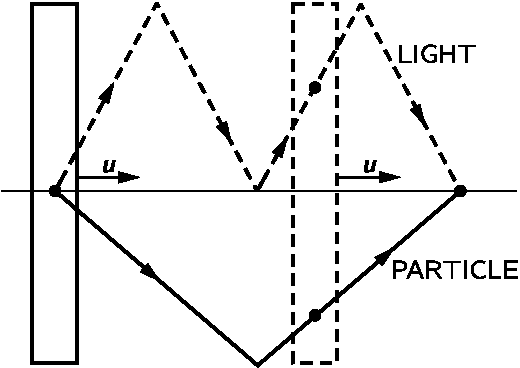
\includegraphics[width=0.7\linewidth]{fyz_fig002.pdf}
      \caption{Trajektorie opisované světelným paprskem a částicí v pohybujících se hodinách
               (\cite[s.~231]{Feynman01})}
      \label{fyz:fig002}
    \end{figure}
    Zjistili jsme, že v soustavě, která je v klidu, je \emph{vertikální složka} rychlosti menší než 
    rychlost světla násobena faktorem \(\sqrt{1 – v^2/c^2}\) (rovnice \ref{FYZ:eq204}). Nyní však 
    předpokládejme, že ve stejných „hodinách“ necháme pohybovat nahoru a dolů nějakou hmotnou 
    částici rychlosti rovnou \(1 /n\) rychlosti světla {obr. \ref{fyz:fig002}). Pokud částice urazí 
    dráhu tam a zpět, urazí světlo tuto dráhu přesně \(n\)-krát. Znamená to, že každé tiknutí 
    „hodin s částicí“ se bude shodovat s \(n\)-tým tiknutím světelných hodin. \emph{To musí platit 
    i tehdy, kdy se celá soustava pohybuje}, neboť fyzikální jev koincidence bude koincidencí v 
    jakékoli soustavě. Protože však rychlost je menší než rychlost světla, musí být i rychlost 
    částice \(v\) menší než odpovídající rychlost ve stejném poměru (s druhou odmocninou)! To je 
    důvod, proč se odmocnina objevuje v každém výrazu pro vertikální rychlost.
    
  \section{Relativistická hmotnost}\label{fyz:IchapXVIsecIV}
    V předcházející kapitole jsme se dověděli, že hmotnost tělesa se zvětšuje se zvyšováním jeho 
    rychlosti. Neuvedli jsme si však žádný důkaz v tom smyslu, že bychom uvažovali podobné 
    argumenty, jako ty o chodu hodin. \emph{Můžeme však} ukázat, že v důsledku relativity a 
    několika dalších rozumných předpokladů, se musí hmotnost měnit právě takto. (Musíme hovořit o 
    „několika dalších předpokladech“, neboť chceme-li provést rozumnou dedukci, nemůžeme nic 
    dokázat, nemáme-li nějaké zákony, o nichž již předpokládáme, že jsou správné.) Abychom se 
    vyhnuli studiu zákonů transformace síly, budeme analyzovat \textbf{srážky}. V tomto případě 
    nepotřebujeme vědět nic o zákonech síly, pouze budeme předpokládat zachování hybnosti a 
    energie. Dále budeme předpokládat, že hybnost pohybující se částice je vektor, který má směr 
    vždy ve směru rychlosti. Nebudeme však předpokládat, že hybnost je rovna násobku nějaké 
    konstanty a rychlosti, jak předpokládal Newton, ale pouze to, že je nějakou funkcí rychlosti. 
    Vektor hybnosti pak napíšeme jako součin určitého koeficientu a rychlosti
    \begin{equation}\label{FYZ:eq211}
      \vec{p} = m_v\vec{v}
    \end{equation}
    Ke koeficientu píšeme index \(v\), abychom si uvědomili, že je funkcí rychlosti a domluvme se, 
    že ho budeme nazývat \uv{hmotností}. Je jasné, že při malých rychlostech to bude tatáž 
    hmotnost, kterou jsme si zvykli měřit. Nyní se pomocí tvrzení, že podle principu relativity 
    musí být fyzikální zákony stejné ve všech souřadnicových soustavách, pokusíme dokázat, že 
    \(m_v\) musí mít tvar \(m_0/(1 – v^2/c^2)\).
    
    \begin{figure}[ht!]  %\ref{fyz:fig001}
      \centering
      \begin{tabular}{cc}
        \subfloat[ ]{\label{fyz:fig001a}
          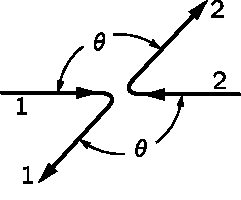
\includegraphics[width=0.35\linewidth]{fyz_fig001a.pdf}}
        \hspace{0.1\linewidth}                                                       &
        \subfloat[ ]{\label{fyz:fig001b}
          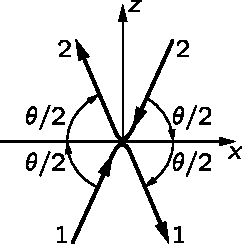
\includegraphics[width=0.35\linewidth]{fyz_fig001b.pdf}}
      \end{tabular}
      \caption{Dva pohledy na pružnou srážku dvou stejných těles pohybujících se stejnou rychlostí 
               v opačných směrech
               (\cite[s.~232]{Feynman01})}
      \label{fyz:fig001}
    \end{figure}
    
    Předpokládejme, že máme dvě částice například dva protony, jež jsou naprosto stejné a jež se 
    pohybují proti sobě přesně stejnou rychlostí. Jejich celková hybnost je rovna nule. Co se s 
    nimi stane? Po srážce musí být směry jejich pohybu navzájem přesně opačné, neboť kdyby tomu tak 
    nebylo, byla by celková hybnost nenulová a hybnost by se nezachovávala. Musí mít stejné i 
    rychlosti, neboť jsou to přesně stejné částice. Musí mít stejnou rychlost jako před srážkou, 
    neboť předpokládáme, že energie se při těchto srážkách zachovává. Takže diagram pružné 
    (reversibilní) srážky bude vypadat jako na obr. \ref{fyz:fig001a}. všechny šipky mají stejnou 
    velikost, všechny rychlosti jsou stejné. Budeme předpokládat, že při takových srážkách se může 
    vyskytnout jakýkoli úhel \(\theta\) a rychlosti si při takové srážce můžeme vybrat 
    libovolně. Dále si všimněme, že otočíme-li souřadnicové osy, může tatáž srážka vypadat jinak. 
    Je výhodné otočit osy tak, že horizontála souměrně rozpůlí diagram (obr. \ref{fyz:fig001b}) .Je 
    to překreslená stejná srážka jako na obr. \ref{fyz:fig001a}, pouze souřadnicové osy jsou 
    pootočené. 

    Nyní docházíme k jádru věci: podívejme se na tuto srážku z hlediska někoho, kdo jede v autě, 
    jehož rychlost je rovna horizontální složce rychlostí první z částic. Jak se mu bude srážka 
    jevit? Bude se mu zdát, že částice 1 se pohybuje přímo nahoru (její horizontální složka 
    zmizela) a pak znovu přímo dolů ze stejného důvodu, tj. bude se jevit jako srážka na obr. 
    \ref{fyz:fig000a}. Avšak částice 2 se pohybovala jinak. Při pohledu z jedoucího auta se bude 
    zdát, že prolétává velkou rychlostí pod menším úhlem (ale úhly před srážkou a po srážce jsou 
    \emph{stejné}). Horizontální složku rychlosti částice 2 označme jako u a vertikální složku 
    rychlostí částice 1 označme jako \(w\).
    
    \begin{figure}[ht!]  %\ref{fyz:fig000}
      \centering
      \begin{tabular}{cc}
        \subfloat[ ]{\label{fyz:fig000a}
          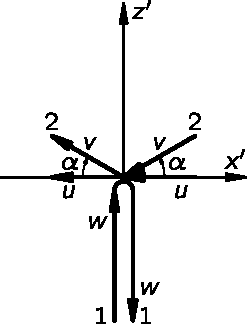
\includegraphics[width=0.4\linewidth]{fyz_fig000a.pdf}}
        \hspace{0.1\linewidth}                                                       &
        \subfloat[ ]{\label{fyz:fig000b}
          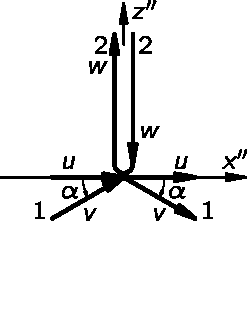
\includegraphics[width=0.4\linewidth]{fyz_fig000b.pdf}}
      \end{tabular}
      \caption{Další dva pohledy na srážku z pohybujících se automobilů
               (\cite[s.~232]{Feynman01})}
      \label{fyz:fig000}
    \end{figure}
    
    Ptáme se, jaká je vertikální rychlost \(u\tan\alpha\)? Kdybychom to věděli, mohli bychom pomocí 
    zákona zachování hybností ve vertikálním směru zjistit hybnost. Je jasné, že horizontální 
    složka hybností se zachovává - před srážkou i po ní, je stejná pro obě částice, přičemž pro 
    částici 1 je nulová. Zákon zachování použijeme proto jen u svislé rychlostí \(u\tan\alpha\). Tu 
    však \emph{můžeme} snadno určit, podíváme-li se na srážku jiným způsobem! Kdybychom srážku 
    pozorovali z auta, které se pohybuje směrem doleva rychlostí \(w\), viděli bychom tutéž srážku, 
    pouze obrácenou naopak, jak je znázorněno na obr. \ref{fyz:fig000b}. Nyní je to částice 2, 
    která letí dolů a nahoru rychlostí \(w\), a částice 1 získala horizontální rychlost \(u\). Teď 
    už víme, jaká je rychlost \(u\tan\alpha\). Je rovna \( w/(1 – u^2/c^2)\) (viz rovnice 
    \ref{FYZ:eq210}). Víme, že změna hybností částice, jež se pohybuje vertikálně, je
    \begin{equation}\label{FYZ:eq212}
      \Delta p = 2m_ww
    \end{equation}
    (proto 2-krát, že máme pohyb nahoru a zpět dolů). Šikmo letící částice má určitou rychlost 
    \(v\), jejíž složky jsou, jak jsme zjistili \(u\) a \( w/(1 – u^2/c^2)\) a jejíž hmotnost je 
    \(m_v\).
    
    \begin{figure}[ht!]  %\ref{fyz_fig125}
      \centering
      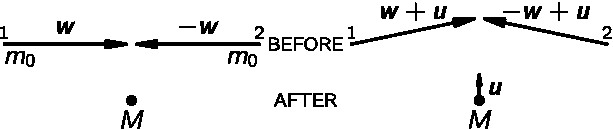
\includegraphics[width=0.7\linewidth]{fyz_fig125.pdf}
      \caption{Dva pohledy na nepružnou srážku dvou těles stejné hmotnosti
               (\cite[s.~233]{Feynman01})}
      \label{fyz_fig125}
    \end{figure}
    
    Změna \emph{vertikální} složky hybností této částice je tedy \(\Delta p' =2m_vw\sqrt{1 – 
    u^2/c^2}\), neboť podle zákona \ref{FYZ:eq211}, je složka hybnosti vždy rovna součinu hmotnosti 
    (odpovídající velikosti rychlosti, jíž se částice pohybuje) a složky rychlosti v daném směru. 
    Tedy, aby byla celková hybnost nulová, musí se vertikální složky hybnosti vyrušit a poměr 
    hmotností částic pohybujících se rychlostí \(v\) a \(w\) musí být proto
    \begin{equation}\label{FYZ:eq213}
      \frac{m_w}{m_v} = \sqrt{1 - \dfrac{u^2}{c^2}}.
    \end{equation}
    
    Vezměme si limitní případ, kdy \(w\) je infinitezimálně malé. Je-li \(w\) skutečně velmi malé, 
    je jasné, že \(v\) a \(w\) jsou prakticky stejné. V tomto případě \(m_w \rightarrow m_0\)  
    \(m_v \rightarrow m_u\). Konečný výsledek je
    \begin{equation}\label{FYZ:eq214}
      m_u = \frac{m_0}{\sqrt{1 - \dfrac{u^2}{c^2}}}.
    \end{equation}
    Bylo by zajímavé provést nyní zkoušku, zda (\ref{FYZ:eq213}) platí pro libovolné hodnoty \(w\), 
    za předpokladu, že (\ref{FYZ:eq214}) je správný vztah pro hmotnost. Všimněme si, že rychlost 
    \(v\), kterou potřebujeme ve vztahu (\ref{FYZ:eq213}) lze vypočítat z pravoúhlého trojúhelníka
    \begin{equation}\label{FYZ:eq215}
      v^2 = u^2 + w^2\left(1 - \dfrac{u^2}{c^2}\right).
    \end{equation}
    Zkouška vychází automaticky, ačkoli jsme (\ref{FYZ:eq214}) odvodili pouze v limitě pro malé 
    \(w\).
    
    Souhlasme nyní s tím, že hybnost se zachovává a že hmotnost závisí na rychlosti podle vztahu 
    (\ref{FYZ:eq214}). Podívejme se, co z toho dále vyplývá. Vezměme \textbf{nepružnou srážku}. Pro 
    jednoduchost předpokládejme, že dvě stejná tělesa, jež se pohybují proti sobě rychlostí \(w\), 
    se srazí, při srážce se spojí a vytvoří nové nehybné těleso (obr. \ref{fyz_fig125} vlevo). 
    Hmotnost každého tělesa odpovídající rychlosti \(w\) je, jak víme, \(m_0\sqrt{1 – w^2/c^2}\) Z 
    předpokladu zachování hybnosti a z principu relativity můžeme dokázat zajímavý fakt týkající se 
    hmotnosti nově vytvořeného tělesa. Představme si nekonečně malou rychlost \(u\) pod pravým 
    úhlem k \(w\) (mohli bychom vzít v úvahu i konečné hodnoty \(u\), ale pomocí nekonečně malých 
    hodnot celou věc snadněji pochopíme) a podívejme se na tuto srážku pohybujíce se ve výtahu 
    rychlostí - \(u\). Co vidíme, je znázorněno na obrázku \ref{fyz_fig125} vpravo. Složené těleso 
    má neznámou hmotnost \(M\). Těleso 1, stejně tak i těleso 2, má svislou složku rychlosti \(u\) 
    a horizontální složku rychlosti, jež je prakticky rovna \(w\). Po srážce se těleso o 
    hmotnosti \(M\) pohybuje nahoru rychlostí \(u\), o níž předpokládáme, že je velmi malá ve 
    srovnání s rychlostí světla i ve srovnání s \(w\). Hybnost se musí zachovávat, proto určíme 
    hybnosti před a po srážce ve svislém směru. Před srážkou máme \(p \sim 2m_wu\) a po srážce je 
    hybnost zřejmě rovna \(p' \sim M_uu\), ale protože \(u\) je tak malé, \(M_u\) je v podstatě 
    rovna \(M_0\). Tyto hybnosti si musí být rovny vzhledem k zachování hybnosti, a proto
    \begin{equation}\label{FYZ:eq216}
      M_0 = 2m_w.
    \end{equation}
    \emph{Hmotnost tělesa vzniklého srážkou dvou stejných těles musí být rovna dvojnásobku 
    hmotností srážejících se těles}. Snad si řeknete: „Ano, je to jasné, to je zachování hmotností. 
    “Jen se neukvapujte říkat „ano, je to jasné“, neboť \emph{hmotnosti těles se zvětšily nad 
    hodnoty hmotnosti, které byly v klidu}, a tak přispívají celkovému \(M\) nejen hmotností, 
    kterou by měly v klidu, ale hmotností větší. Zdá se to být překvapující, ale aby při srážce 
    dvou těles platil zákon zachování hybností, musí být hmotnost výsledného tělesa větší, než jsou 
    klidové hmotnosti obou těles, ačkoli po srážce jsou tato tělesa v klidu!
    
  \section{Relativistická energie}\label{fyz:IchapXVIsecV}
    V poslední kapitole jsme dokázali, že v důsledku závislosti hmotnosti na rychlosti a v důsledku 
    Newtonových zákonů vychází, že změna kinetické energie způsobená celkovou prací sil je vždy
    \begin{equation}\label{FYZ:eq217}
      \Delta T = (m_u - m_0)c^2 = \frac{m_0c^2}{\sqrt{1 - \dfrac{u^2}{c^2}}} - m_0c^2.
    \end{equation}
    Šli jsme dokonce i dále a zjistili jsme, že celková energie je rovna „celkové hmotnosti krát 
    \(c^2\)“. Nyní budeme v diskuzi pokračovat.
    
    Předpokládejme, že uvnitř tělesa \(M\) můžeme stále vidět naše dvě tělesa o stejných 
    hmotnostech, která se srazila. Například proton a neutron se „spojily“, ale stále se ještě 
    pohybují uvnitř \(M\). I když by se zpočátku zdálo, že hmotnost  \(M\) bude rovna \(2m_0\), 
    zjistili jsme, že je rovna \(2m_w\) a ne \(2m_0\). Protože vstupní hmotnost je \(2m_w\) a 
    klidová hmotnost vnitřních částic je \(2m_0\), je \emph{přebytečná} hmotnost složené částice 
    rovna dodané kinetické energii. To znamená, že energie má setrvačnou hmotnost. V předcházející 
    kapitole jsme hovořili o zahřívání plynu. Molekuly plynu se pohybují a pohybující se tělesa 
    jsou těžší, proto dodáváme-li plynu energii, pohybují se jeho molekuly rychleji a plyn se stává 
    těžším. Tento argument je ve skutečnosti úplně obecný a z naší diskuze o nepružném rozptylu 
    vyplývá, že dodatečná hmotnost existuje, ať už je, nebo není \emph{kinetickou} energií. Jinými 
    slovy, jestliže se dvě částice spojí a získají potenciální energii nebo jakýkoli jiný druh 
    energie, jestliže se zpomalí tím, že se budou pohybovat do kopce, prací proti vnitřním silám 
    nebo čímkoli jiným, platí stále, že hmotnost odpovídá celkové dodané energii. Vidíme, že 
    odvozené zachování hmotnosti je ekvivalentní zachování energie, a proto v teorii relativity 
    není místo pro čistě nepružné srážky, jak tomu bylo v Newtonově mechanice. Podle Newtonovy 
    mechaniky se dvě částice mohou srazit, přičemž vznikne částice s hmotností \(2 m_0\), která se 
    vůbec neliší od částice, jež by vznikla, kdyby se původní částice spojily velmi pomalu. 
    Samozřejmě, ze zákona zachování energie víme, že uvnitř bude větší kinetická energie, ale podle 
    Newtonových zákonů to neovlivňuje hmotnost. Nyní však víme, že to není možné - výsledná částice 
    bude \emph{těžší} díky kinetické energii srážky, a proto to bude \emph{jiná} částice. 
    Spojíme-li částice jemně, vznikne něco s hmotností \(2m_0\) a spojíme-li je násilně, vznikne 
    částice s větší hmotností. Tuto změnu hmotnosti umíme \emph{zjistit}. A tak nutně proto v 
    teorii relativity musí jít zachování energie ruku v ruce se zachováním hybností.
    
    Z toho vyplývají zajímavé důsledky. Předpokládejme například, že máme těleso s naměřenou 
    hmotností \(M\) a cosi způsobí, že se rozletí na dvě stejné části pohybující se rychlostí \(w\) 
    tak, že každá má hmotnost \(m_w\). Dále předpokládejme, že tyto části budou mít v cestě 
    dostatek materiálu, který je zpomalí, až se zastaví. Jejich hmotnost bude \(m_0\). Jak velkou 
    energii odevzdaly materiálu, když se zastavily? Podle výše dokázané teorie bude příspěvek každé 
    části \((m_w – m_0)c^2\). Takové množství energie zůstává v materiálu ve formě tepla, 
    potenciální energie atd. Protože \(2m_w = M\), uvolněná energie \(E = (M - 2m_0)c^2\). Podle 
    této rovnice se například odhadlo, kolik energie by se uvolnilo při štěpení jader v atomové 
    bombě. (Ačkoli úlomky štěpení nejsou přesně stejné, lze je za takové zhruba považovat.) 
    Hmotnost atomů uranu byla známa (byla změřena dávno předtím) a také z hmotnosti atomů, na které 
    se rozpadávají (jodu, xenonu atd.), byly známé. Hmotností nerozumíme hmotnost po dobu pohybu, 
    ale hmotnosti atomů, když jsou v \emph{klidu}. Obě veličiny \(M\) i \(m_0\) jsou tedy známé. 
    Odečtením těchto dvou čísel lze vypočítat, jaká energie se uvolní, když se \(M\) rozštěpí na 
    dvě „poloviny“. Toto byl důvod, proč ve všech novinách nazývali starého dobráka Einsteina 
    „otcem“ atomové bomby. Ve skutečnosti tím bylo myšleno, že kdybychom mu oznámili, o jaký proces 
    půjde, mohl by nám již před časem říci, jaká energie by se uvolnila. Energie, která by se mohla 
    uvolnit při rozštěpení atomu uranu, byla určena asi šest měsíců před prvním přímým pokusem. 
    Jakmile se tato energie uvolnila, kdosi ji změřil přímo (a i kdyby Einsteinův vzorec nebyl 
    správný, i tak by ji byli každopádně změřili). A od okamžiku, kdy ji změřili, vzorec už dále 
    nepotřebovali. Samozřejmě, tím nechceme snižovat Einsteinovy zásluhy, spíše chceme kritizovat 
    noviny a populární líčení rozvoje fyziky a techniky. Problém, jak docílit toho, aby proces 
    uvolnění energie probíhal efektivně a rychle, nemá se vzorcem nic společného.
    
    Tento výsledek je stejně významný i pro chemii. Kdybychom například zvážili molekulu oxidu 
    uhličitého a porovnali ji s hmotností uhlíku a kyslíku, mohli bychom zjistit, jaká energie by 
    se uvolnila při vzniku oxidu uhličitého z kyslíku a uhlíku. Jediným problémem je, že rozdíly 
    hmotností jsou tak malé, že po technické stránce je měření velmi obtížně uskutečnitelné.
    
    Vraťme se ještě k otázce, zda bychom mohli přidávat \(m_0c^2\) ke kinetické energii a od této 
    chvíle říkat, že celková energie tělesa je \(mc^2\) Za prvé, kdybychom mohli uvnitř \(M\) stále 
    \emph{vidět} složky s klidovou hmotností, mohli bychom říci, že hmotnost \(M\) složeného tělesa 
    se zčásti skládá z klidové energie hmotnosti příslušných složek, zčásti z kinetické energie 
    těchto složek a zčásti z jejich potenciální energie. V přírodě jsme však objevili různé 
    částice, které podléhají právě takovým reakcím, o jakých jsme již hovořili a v nichž navzdory 
    všemu studiu \emph{nemůžeme vidět vnitřní části} Například \(K\) mezon se rozpadá na dva piony 
    podle zákona (\ref{FYZ:eq216}), ale říci, že se skládá ze dvou pionů, je nevhodné, neboť někdy 
    se rozpadá na tři piony!
    
    Proto máme \emph{novou ideu}: Nemusíme vědět, jak vypadají částice zvnitřku. Nemůžeme, a ani 
    nepotřebujeme, zjišťovat uvnitř částice, jaká část energie je klidová energie částí, na něž se 
    částice chystá rozpadnout. Není vhodné, a často ani možné, rozdělit celkovou energii tělesa 
    \(mc^2\) na klidovou energii vnitřních částic, jejich kinetickou a potenciální energii. Místo 
    toho prostě hovoříme o \emph{celkově energii} částice. Přidáváním konstanty \(m_0c^2\) ke všemu 
    „posouváme odečet“ energie a říkáme, že celková energie částice je rovna součinu hmotnosti v 
    pohybu a \(c^2\). Je-li těleso v klidu, je energie rovna součinu klidové hmotnosti a \(c^2\).
    
    Nakonec si ukážeme, že rychlost \(v\), hybnost \(p\) a celková energie \(E\) navzájem souvisejí 
    jednoduchým způsobem. Skutečnost, že hmotnost při rychlosti \(v\) je rovna hmotnosti \(m\) 
    dělené \(\sqrt{ 1 – v^2/c^2}\) se používá překvapivě zřídka. Místo toho lze snadno dokázat tyto 
    vztahy
    \begin{align}
      E^2 - p^2c^2 = m_0^2c^4   \label{FYZ:eq218}  \\
      \shortintertext{a}
      pc = E\frac{v}{c},        \label{FYZ:eq219}
    \end{align}
    jež jsou velmi užitečné a používají se častěji. 
    
  \section{Příklady a cvičení}\label{fyz:IchapXVIsecVI}

} %tikzset
%---------------------------------------------------------------------------------------------------
\printbibliography[heading=subbibliography]
\addcontentsline{toc}{section}{Seznam literatury}